\section{Um pouco de geometria}

Todo mundo sabe que a área de um quadrado é dado pelo quadrado de sua aresta, $A=a^2$. O perímetro por sua vez é um múltiplo da aresta, $P = 4\cdot a$. No caso de uma circunferência de raio $r$, $A = \pi r^2$ e $P = 2\pi r$. Em geral qualquer figura geométrica apresenta relações do tipo 
\[
\frac{A}{L^2} = k_1 \qqrq \frac{P}{L} = k_2
\]
de modo que a razão entre a área e uma dimensão característica ao quadrado é uma constante e a razão entre perímetro e esta mesma dimensão característica também é constante. 

Este tipo de relação continua valendo para figuras compostas mais complexas como a dada na figura \ref{fig:L2d} que mostra uma geometria um pouco mais complexa, composta por dois retângulos. Neste caso, a área é $A = a\cdot b + c\cdot d$ e o perímetro é $a + 2b + 2d + c$. Novamente esta figura geométrica pode ser especificada usando o lado $a$ e três parâmetros $\alpha_1$, $\alpha_2$ e $\alpha_3$ onde
\[
b = \alpha_1\cdot a, \qquad d = \alpha_2\cdot a, \qquad c = \alpha_3\cdot a
\]
A área e o perímetro desta figura geométrica são dadas por:
\[
\frac{A}{a^2} = (\alpha_1 + \alpha_2\cdot\alpha_3) \qquad \frac{P}{a} = (1 + 2\alpha_1+2\alpha_2+\alpha_3)
\]
o que se percebe é que existe um padrão, a cada figura geométrica, pode-se associar uma escala $a$ e com a ajuda de outros parâmetros pode-se definir funções como área e perímetro de modo que 
\[
\frac{P}{a} = f(\alpha_1, \alpha_2, \alpha_3, \ldots) \qquad \frac{A}{a^2} = g(\alpha_1, \alpha_2, \alpha_3, \ldots)
\]

\begin{figure}
\centering
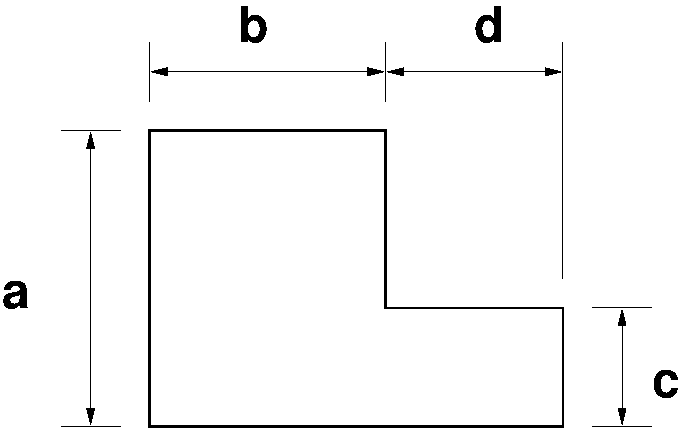
\includegraphics[width=0.6\textwidth]{./figuras/L2d.pdf}
\caption{Figura geométrica composta por dois retângulos}
\label{fig:L2d}
\end{figure}

Ao se multiplicar todas as dimensões características de um figura geométrica por uma constante, ou seja, na figura \ref{fig:L2d}, multiplicar $a$ por esta constante, o perímetro varia linearmente com esta constante e a área varia com o seu quadrado. Escolhendo $a'=k\cdot a$, a área $A'$ e perímetro $P'$ desta nova figura geométrica têm o seguinte valor:

\[
P' = \frac{a'}{a}\cdot P = k\cdot P \qquad A' = \left(\frac{a'}{a}\right)^2\cdot A = k^2\cdot A
\]

As grandezas que permanecem constantes quando se muda a escala da figura geométrica são parâmetros adimensionais.

\subsection{Teorema de pitágoras}

\begin{figure}
  \centering
  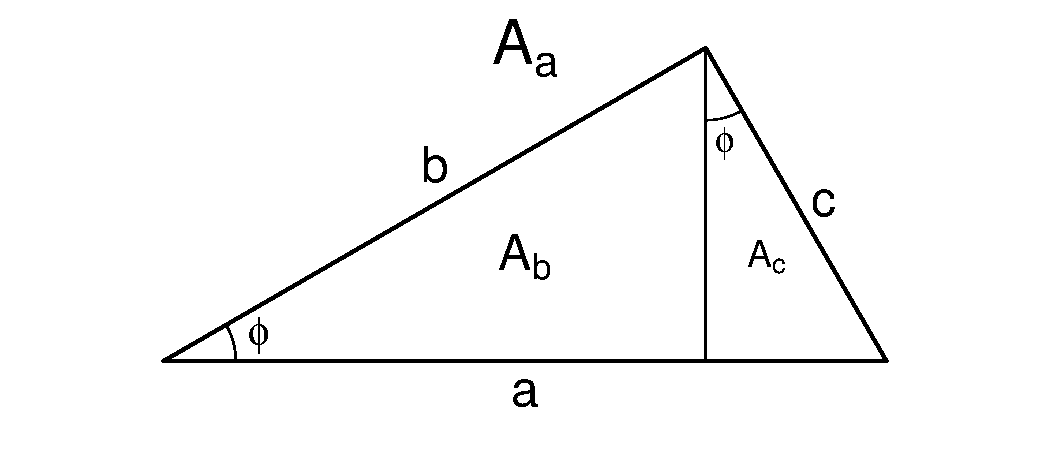
\includegraphics[width=0.9\textwidth]{./figuras/pitagoras}
  \caption{Teorema de Pitágoras}
  \label{fig:pit}
\end{figure}

Dois triângulos são semelhantes se dois ângulos são iguais. Se um dos ângulos é reto, o triângulo é chamado de de triângulo retângulo. Se a hipotenusa for escolhida como dimensão característica e o ângulo entre a hipotenusa e um cateto for denominado por $\phi$, a área deste triângulo é dada por uma relação do tipo
\[
A(h,\phi) = h^2\cdot f(\phi)
\]
A figura mostra como um triângulo retângulo pode ser dividido em dois triângulos retângulos semelhantes (mesmo ângulo $\phi$). Nesta subdivisão, 
\[
A_a a^2\cdot f(\phi) = A_b + A_c = b^2\cdot f(\phi) + c^2\cdot f(\phi)
\]

Dividindo por $f(\phi)$ chega-se ao teorema de Pitágoras:
\[
a^2 = b^2 + c^2
\]

Para concluir, esta demonstração do teorema de Pitágoras é resultado do fato de que a área de um triângulo é o produto entre hipotenusa ao quadrado e uma função do ângulo de um dos vértices, que não muda com a escala.


\subsection{Floco de Koch}

As relações anteriores contnuam válidas no caso de figuras geométricas mais ``exóticas''. A figura \ref{fig:koch} mostra um floco de Koch

\begin{figure}
\centering
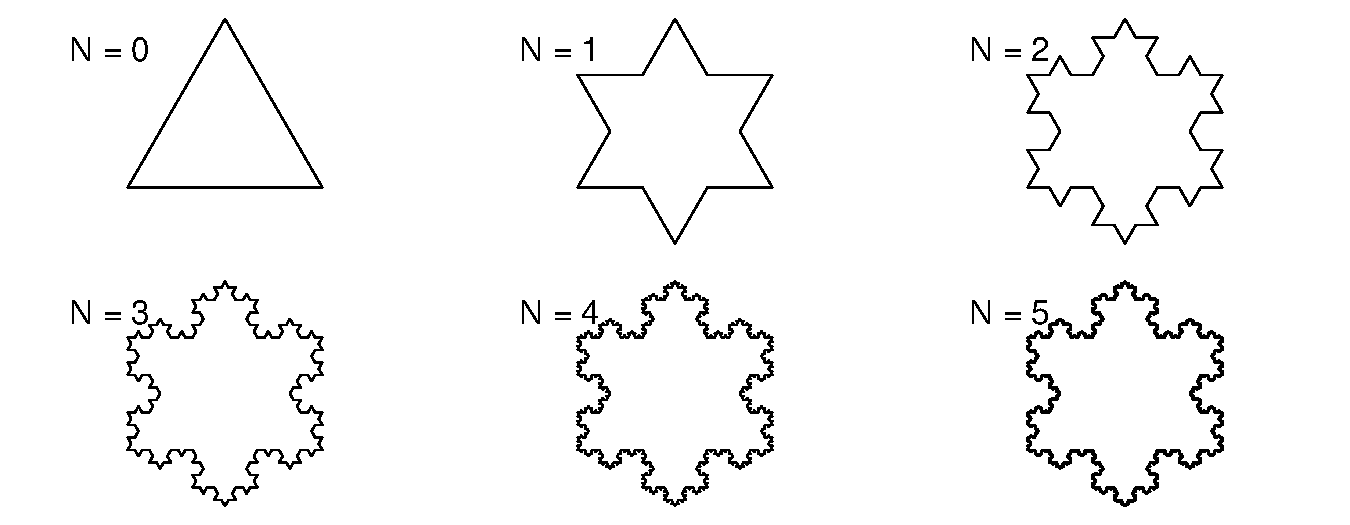
\includegraphics[width=\textwidth]{./figuras/koch.pdf}
\caption{Desenvolvimento do floco de Koch.}
\label{fig:koch}
\end{figure}

A área e perímetro do floco de Koch dependem da dimensão básica $L$ (lado do triângulo original) e o número de vezes $N$ que o floco é refinado. A área e o perímetro é dado por:
\[
\frac{A}{L^2} = \frac{\sqrt{3}}{20} \cdot \left[8 - 3\left(\frac{4}{9}\right)^N\right] \qrq \frac{P}{L} = 3\cdot\left(\frac{4}{3}\right)^N
\]
É interessante observar que no limite $N\lra\infty$ a área chega a um limite finito mas o mesmo não ocorre com o perímetro que sempre aumenta:

\[
\lim_{N\lra\infty} \frac{A}{L^2} = \frac{2}{5}\sqrt{3} \qquad\qquad \lim_{N\lra\infty}\frac{P}{L} = \infty
\]

Mas mesmo neste caso as regras dimensionais envolvendo a área e o perímetro continuam valendo se $N$ for fixado. Por outro lado se $N$ pode variar as relações anteriores indicam que aproximações são possívei em algum caso. Se o fenômeno em questão depender da área, basta escolher $N$ grande o suficiente. Já se depender do perímetro talvez seja necessário especificar $N$.

Este tipo de geometria pode parecer uma curiosidade matemática mas a natureza está repleta de coisas deste tipo. Qual o comprimento da costa do Brasil? Richardson (o mesmo da cascata de energia da turbulência, meteorologia computacional, etc) tentou determinar o comprimento da costa do Reino Unido e chegou em relações como a anterior. Qual a fronteira de uma nuvem? Em uma camada limite turbulenta, qual a geometria que separa o escoamento externo potencial do escoamento turbulento?

O floco de Koch também apresenta uma outra característica interessante e importante: auto-semelhança. A figura \ref{fig:koch-self} mostra vistas explodidas de uma seção do floco de Koch. Repare que os padrões se repetem em diferentes escalas. A auto-semelhança é observada em escalas intermediárias. Nas maiores escalas (muito maiores que o floco) ela deixa de ser observada. Nas menores escalas chegamos à resolução da figura e a auto-semelhança se perde. 

\begin{figure}
\centering
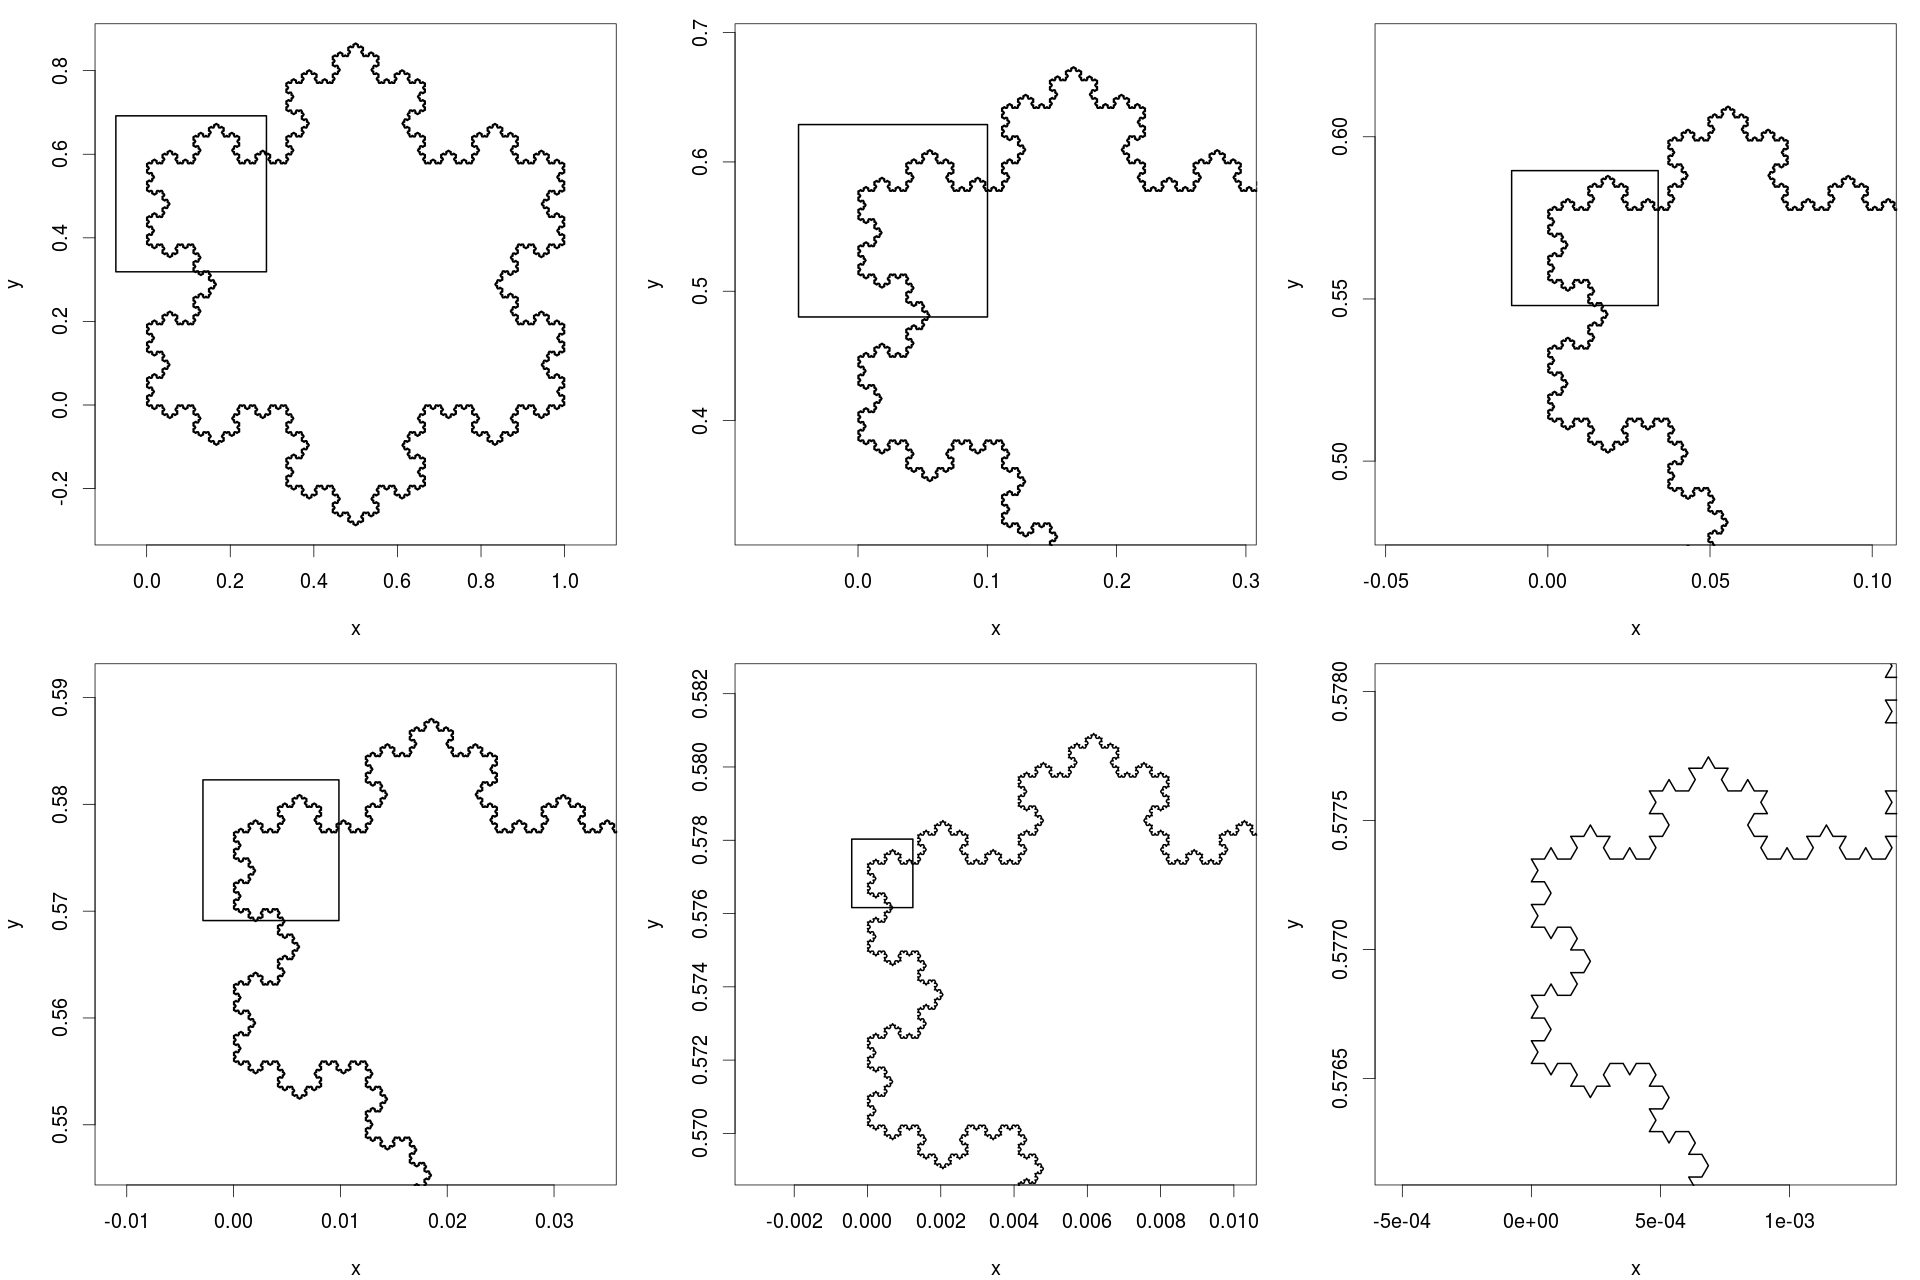
\includegraphics[width=1\textwidth]{./figuras/koch-self.png}
\caption{Auto-semelhança no floco de Koch.}
\label{fig:koch-self}
\end{figure}


O fenômeno da auto-semelhança não está restrita a geometrias exotéricas e fenômenos complexos. Sempre que leis de potência existirem, será observado auto-semelhança, como se vê na figura \ref{fig:power-law} onde a lei de potência 
\[
y = x^\frac{5}{2}
\]
é observada em diferentes escalas. Visualmente nada muda.

\begin{figure}
\centering
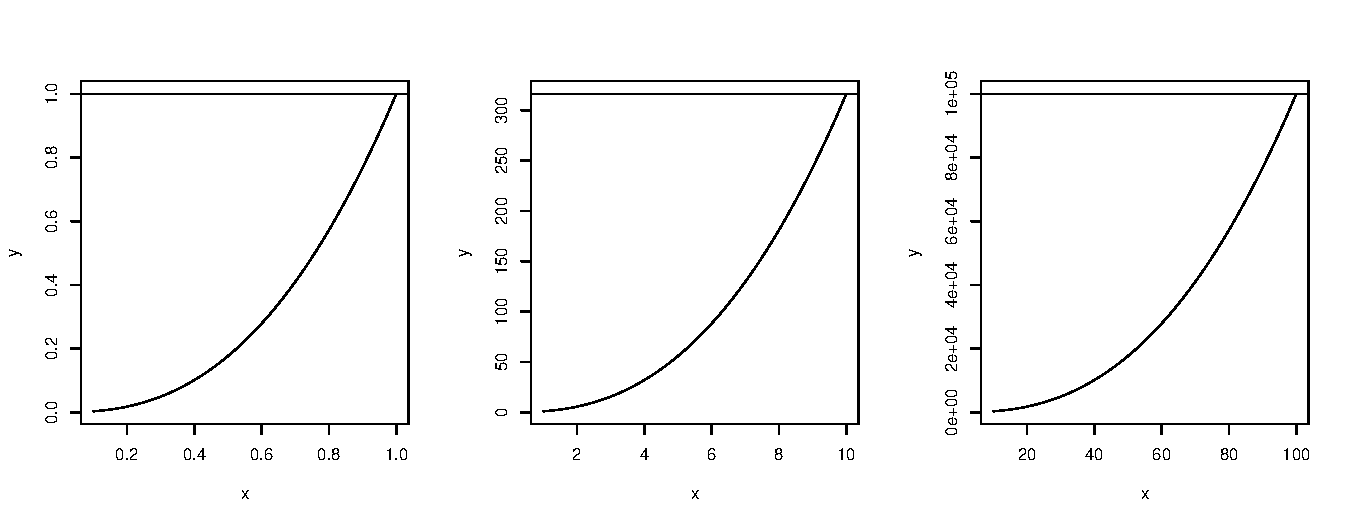
\includegraphics[width=\textwidth]{./figuras/power.pdf}
\caption{Auto-semelhança em leis de potência. A curva $y = x^{5/2}$ em diferentes escalas.}
\label{fig:power-law}
\end{figure}

